
\documentclass[11pt, a4paper]{article}
\usepackage{graphicx}
\usepackage{amsmath}
\usepackage{listings}


\title{Assignment No 8} % Title

\author{SUHAS C EE20B132} % Author name

\date{\today} % Date for the report
\begin{document}		
		
\maketitle % Insert the title, author and date
\section{Aim}
%Create new section;it is autonumbered
The aim of this assignment is to examine the DFT of various functions using the fft library in numpy.
 
\section{Spectrum of $sin^3(t)$ and $cos^3(t)$}
The signals can be represented as follows:
\begin{equation}
\sin^3(t) = \frac{3}{4}\sin(t) - \frac{1}{4}\sin(3t)
\end{equation}
\begin{equation}
\cos^3(t) = \frac{3}{4}\cos(t) + \frac{1}{4}\cos(3t)
\end{equation}
\begin{figure}[!tbh]
   	\centering
   	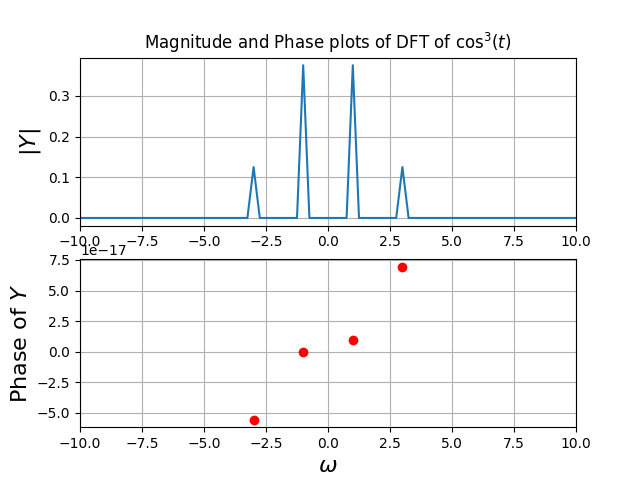
\includegraphics[scale=0.5]{figure1.png}  % Mention the image name within the curly braces. Image should be in the same folder as the tex file. 
   	\caption{DFT of $cos^3(t)$}
   	\label{fig:sample}
   \end{figure} 
 \begin{figure}[!tbh]
   	\centering
   	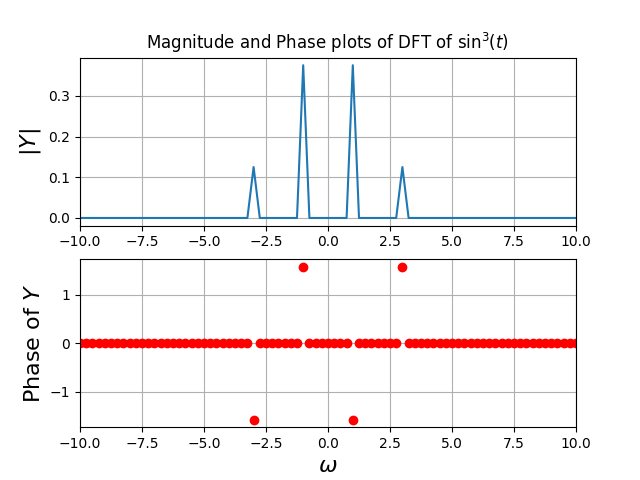
\includegraphics[scale=0.5]{figure0.png}  % Mention the image name within the curly braces. Image should be in the same folder as the tex file. 
   	\caption{DFT of $sin^3(t)$}
   	\label{fig:sample}
   \end{figure} 
Thus there will be 4 impulses in the frequency spectrum. Following are the spectrums obtained.

\newpage
\section{Frequency Modulation}
Consider the frequency modulated signal, $\cos(20t + 5\cos(t))$
\begin{figure}[!tbh]
   	\centering
   	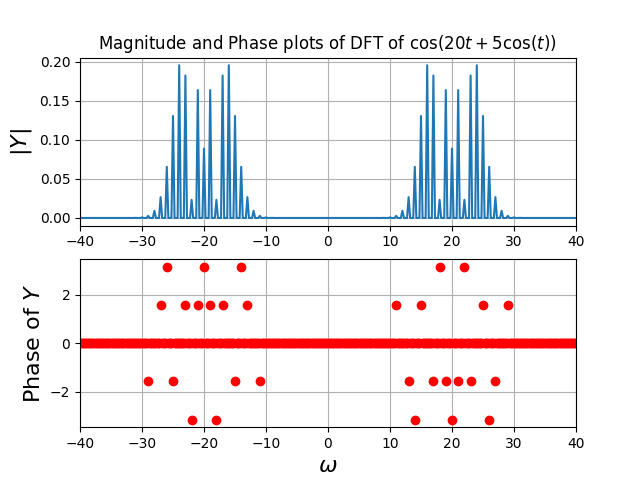
\includegraphics[scale=0.5]{figure2.png}  % Mention the image name within the curly braces. Image should be in the same folder as the tex file. 
   	\caption{DFT of fm signal}
   	\label{fig:sample}
   \end{figure} 
   
   
\newpage
\section{Gaussian}
The Gaussian function $f(x) = e^{-x^2/2}$ is not band limited as the frequency spectrum has non zero values even for large frequencies.
The value of error varies with different time ranges and the sampling rate. For sampling rate = 512 and time range = $8\pi$ s, the error is found to be around $10^{-15}$.
As the sampling rate increases, the peak sharpens. Also, it broadens for greater time ranges.
\begin{figure}[!tbh]
   	\centering
   	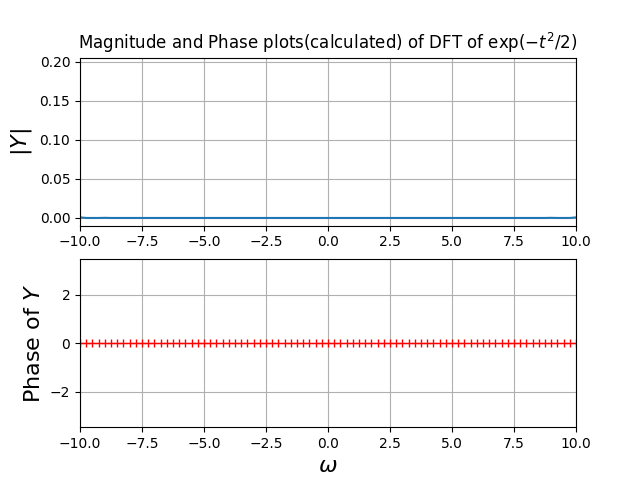
\includegraphics[scale=0.5]{figure3.png}. 
   	\caption{Magnitude and Phase plots(calculated) of DFT of  \exp(-t^{2}/2)}
   	\label{fig:sample}
   \end{figure} 


\begin{figure}[!tbh]
   	\centering
   	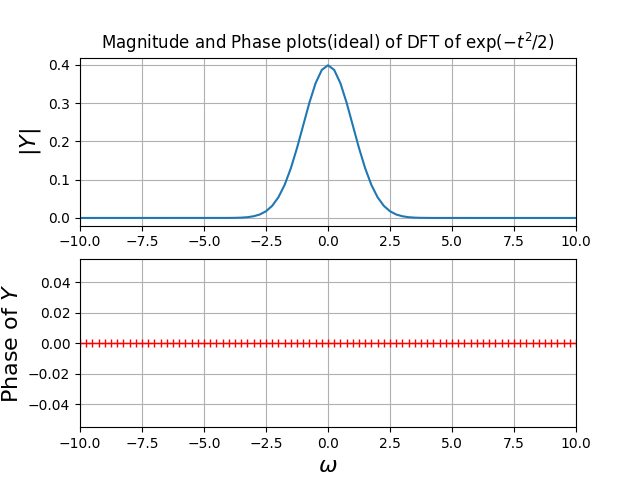
\includegraphics[scale=0.5]{figure4.png}  
   	\caption{Magnitude and Phase plots(ideal) of DFT of  \exp(-t^{2}/2)}
   	\label{fig:sample}
   \end{figure}
   
\section{CONCLUSION}
From the above pairs of plots, it is clear that with a sufficiently large window size and sampling
rate, the DFT approximates the CTFT of the gaussian.

 Sampling after windowing is done so that the DFT can be calculated using the Fast Fourier
Transform. This is then a sampled version of the DTFT of the sampled time domain signal.

With sufficiently large sampling rates, this approximates the CTFT of the original time
domain signal.

This process is done on the gaussian and the results are in agreement with what is expected

\end{document}
